\documentclass[•]{standalone}

\usepackage{pgfplots}
\usepackage{tikz}
\usepackage{trfsigns}

\begin{document}

\begin{tikzpicture}[scale=.9]

\draw[line width = .4cm] (-1,0)--++(30:1)coordinate(help);
\draw[thick] (help)--++(30+90:.5)--++(30:.5)--++(-60:1)--++(-150:.5)--cycle;
\draw[thick,->] (help)++(50:.8)arc(50:10:.8);
\draw[fill=gray] (0,0)rectangle(1,-1);

% Rohdaten
\path (-5,-3)node(InAnalog){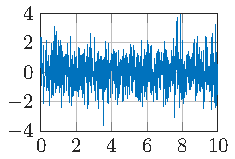
\includegraphics[width=3.5cm]{Matlab/x.pdf}};
\path (InAnalog.west)node[left]{IN};
\path (5,-3)node(OutAnalog){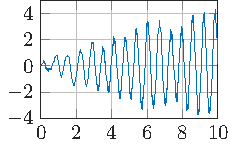
\includegraphics[width=3.5cm]{Matlab/y.pdf}};
\path (OutAnalog.east)node[right]{OUT};
\draw[->] (-1,0)--(InAnalog);
\draw[->] (1,-.5)--(OutAnalog);
\path (0,-3)node{Analoge Signale};

% Rohdaten gefiltert
\path (-5,-7)node(Infilt){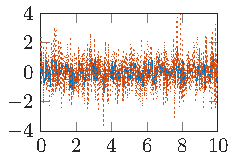
\includegraphics[width=3.5cm]{Matlab/xfilt.pdf}};
\path (Infilt.west)node[left]{IN};
\path (5,-7)node(Outfilt){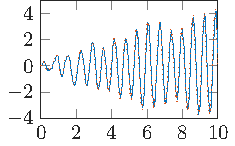
\includegraphics[width=3.5cm]{Matlab/yfilt.pdf}};
\path (Outfilt.east)node[right]{OUT};
\path (0,-7)node[align=center]{Lowpass Filter \& AD-Wandler \\ (Anti - Aliasing)};
\path (0,-5.2)node(Lowpass){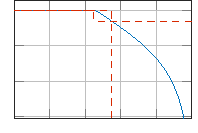
\includegraphics[width=3.5cm]{Matlab/Lowpass.pdf}};
\draw[->] (InAnalog)--(Lowpass);
\draw[->] (Lowpass)--(Infilt);
\draw[->] (OutAnalog)--(Lowpass);
\draw[->] (Lowpass)--(Outfilt);

% Rohdaten gefenstert
\path (-5,-11)node(InWin){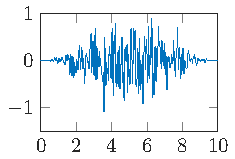
\includegraphics[width=3.5cm]{Matlab/xfiltw.pdf}};
\path (InWin.west)node[left]{IN};
\path (5,-11)node(OutWin){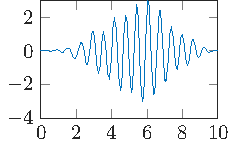
\includegraphics[width=3.5cm]{Matlab/yfiltw.pdf}};
\path (OutWin.east)node[right]{OUT};
\path (0,-11)node[align=center]{Anwenden von Fenster Fkt \\ (Anti - Leakage)};
\path (0,-9.2)node(window){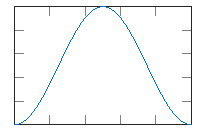
\includegraphics[width=3.5cm]{Matlab/window.pdf}};
\draw[->] (Infilt)--(window);
\draw[->] (window)--(InWin);
\draw[->] (Outfilt)--(window);
\draw[->] (window)--(OutWin);

% FFT
\path (-5,-15)node(InFFT){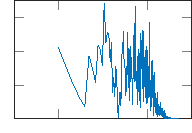
\includegraphics[width=3.5cm]{Matlab/xfiltwfft.pdf}};
\path (InFFT.west)node[left,align=right]{IN \\ SPEC \\ $|X(j\omega)|$};
\path (5,-15)node(OutFFT){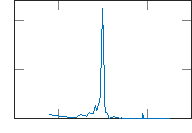
\includegraphics[width=3.5cm]{Matlab/yfiltwfft.pdf}};
\path (OutFFT.east)node[right,align=left]{OUT \\ SPEC \\ $|Y(j\omega)|$};
\path (0,-15)node{Berechne FFT};
\path (0,-13.5)node[rectangle,draw](FFT){FFT};
\draw[->] (InWin)--(FFT);
\draw[->] (FFT)--(InFFT);
\draw[->] (OutWin)--(FFT);
\draw[->] (FFT)--(OutFFT);

% Uebertragungfunktion
\path (0,-20)node(G){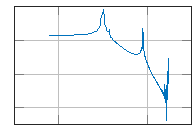
\includegraphics[width=5cm]{Matlab/G.pdf}};
\draw[->] (OutFFT)--(G);
\draw[->] (InFFT)--(G);
\path (G.south)node[below]{Berechne FRF};
\path (G.east)node[right]{FRF $= \frac{|Y(j\omega)|}{|X(j\omega)|}$};

\end{tikzpicture}

\end{document}